\title{Theory}

\documentclass[11pt]{article}
\usepackage[utf8]{inputenc}
\author{
        Kasper Videbæk \\
}
\date{\today}
 \usepackage{amsmath}
\usepackage{graphicx}
\usepackage[numbers]{natbib}
\usepackage{todonotes}
\usepackage[hidelinks]{hyperref}
\usepackage{epstopdf}
\usepackage{wrapfig}
\usepackage[noend]{algpseudocode} 
\usepackage{algorithm}
\renewcommand{\algorithmicforall}{\textbf{for each}}

\begin{document}
\maketitle

\tableofcontents

\clearpage 
\section{Introduction}

\clearpage 
\section{Theory}
Several topics, scientific as well as practical, are related to the work that will be done in this thesis.

In this section we will give a brief overview of what areas we will be going through, and what related work has already been done in those areas. In the first subsection we will look into research that already have worked on embedding syntax tree knowledge into version control systems, and in the second section, we will look into tree differencing. In the last section we will look into general knowledge about merging trees.

\subsection{Version control systems}
The overall goal of version control systems is to support development of documents, by keeping track of changes over time. In the context of software development, version control systems are frequently used to keep track of source code. Two overall groups of version control systems exists: Distributed and centralized. In the context of this thesis, we do not distinguish between these two - but abstract all the different merging-scenarios possible into the simple concept of merging two branches with a common ancestor.\todo[inline]{Skrive mere om process?}

Merging in version controls is the process of producing a single file, given two files that have evolved in different directions from a common ancestor. Merging source code is an inherent part of software development, and has gone through some development and automation since the first version control systems. Merging algorithms generally work by matching content between the two branches and the common ancestor. Given these matchings it is possible to merge the content into one common child. If this is not possible, we have a conflict and it will be presented to the user.

Merging tools of version control systems are mostly line based and oblivious to the structure of the content of the files contained. They work by matching each line in the two branches with the common ancestor. Given these matchings, it will conclude which lines has been deleted and added in the two different branches, and produce single file that has all these deletions ans insertions included. If changes happen near each other, it will produce a conflict.

%Version control systems can contain any type of file. Binary files are generally not merged by version control systems. Instead they are treated as conflicts instantly. 

A line based approach to works relatively well with source files and XML files, since line breaks are often used to make the structure of the code more easily readable for users. It is common for XML files to have opening and closing XML-tags on their own lines, and conventions of most programming languages have only one statement per line and opening block on lines of their own. In some programming languages line breaks are actually a part of the structure of the code - which makes them even more suitable for this approach.

However conventions of XML or source code can be broken. An entire XML-file can be a single line, and have the exact same meaning. Likewise with most source code - a function body can be written on a single line in many programming languages, and the compiler will never notice.

\todo[inline]{Er formålet med dette speciale at fixe "ikke bruger-læsbar-merging"?}

A structured merging approach will clearly be helpful for files that are not structured with line breaks. However this is not a very common case. The better case for improving version control by introducing structural knowledge, is where a single line contains structure. \todo[inline]{Dette hører nok til et andet sted}

A conflict can be defined in quite a few ways for line based tools. In the Unix tool diff3, a conflict is a sequence of lines, that is changed in both branches, and is not separated by a single line that is unchanged in both branches. Such a conflict detection scheme is clearly an approximation. It is oblivious to the structure of the data and one could craft input that will output invalid structural data. Further, the  actual meaning of the merged data is not considered at all - even if it is structurally valid, it might semantically be nonsense, even though a conflicts is not produced.


\subsection{Automatic merging}
The reason merging tools are still line based, can probably be attributed to such an approach working relatively well with source code, XML and other files often found in repositories. Structure matching will most definitely also be a more time consuming task, and given the general use case of commits in version control, it might not be worth the extra computation time. Further programs are generally undecidable which means it would be impossible to actually decide if a merge will work as intended by the user.

One very commonly used algorithm for merging is Diff3. \citet{Khanna} investigated it formally by regarding a file as a sequence where each line was an item in the sequence. They set up a number of expectations of what you would expect from a merge, and showed that many of these assumptions does not hold: Conflicts can happen even when only unrelated regions are changed, differencing after a merge does not produce empty output, merging fails when both branches are very different from the ancestor and so forth. Even though this is the case, Diff3 continues to be widely used with few complaints of it shortcomings - it seems that the situations where Diff3 breaks are quite uncommon in version control systems.

Common algorithms for merging are state based. They compare the final state of branches, and creating a series of operations that will transform one document from one state into another. \citet{Lippe} described a different approach, where editing tools instead would remember the operations used to transform the data, and where the merge process will be a matter of applying these transformations in the right order to minimize the amount of conflicts.

\todo[inline]{Mention whitespace ignoring}
\todo[inline]{Mention horizontal differincing}
\todo[inline]{Talk about prettyprinters.}
\todo[inline]{Point out that merges might not compile.}


\subsection{Programming languages}
Programming languages are abstractions over the calculations computers can perform. They makes it easier for a programmer to express the problems they need to solve, without requiring the programmer to handle intricate details about memory and processors, and they allow the user to write programs as text files, and let the computer handle the process of executing the ideas expressed in the code.

In this section we will look into the process that a program goes through in the process up until execution, to give a simple overview of how this process gets us to syntax trees, and to look into what kind of consequences a this process has from regenerating concrete syntax when given a syntax tree.

\subsubsection{Grammars}
The process of turning programs into execution often relies on lexers and parsers. A lexer divides a programs into tokens. A token is any concrete string of text that is legal at any point in the program text. It can be numbers, strings, keywords, parenthesis, and any other character or sequence of characters that is legal at some point in the program text. 

After the lexer has divided the program into tokens, these are passed to the parser. The parser contains a set of rules that are possibly allowed token sequences - it defines whether or not a given token is valid. Given a grammar of a language, we will be able to to parse the syntax of a legal program, or to generate syntax errors for invalid ones. While parsing it will be possible to visit each part of the concrete syntax, making the construction of a syntax tree possible.

\subsubsection{Syntax Trees}
The purpose of parsing source code is often iterating over the elements of it to generate a syntax tree. A syntax tree is a tree representation of the program. The syntax tree representation is useful for further processing of the semantics of a program. At this point a lot of details about the concrete textual representation of the code has also left behind.

Depending on what kind of choice of syntax tree is done, information of the concrete syntax might be lost - several grammatical rules might produce the exact same syntax node.

In C, for example, the construct \texttt{a[i]]} is a shorthand for \texttt{*(a + i)} and should produce the same semantic behaviour. Rewriting them both into the same structure in the syntax tree is one way to resolve this. Doing this also means that given a syntax tree it will be harder, or impossible, to determine what the concrete syntax was.

Given the purpose of this thesis, the choice of syntax tree is quite important for us: We will be looking at syntax nodes, and want to generate concrete syntax - which means we will always want a syntax tree that is as closely corresponding to the grammatical constructs of the language.

\subsubsection{Pre-processing and comments}
\todo[inline]{Syntax Trees and Preprocessing??}
%http://bartho.net/publications/Adding_preprocessor_directives.pdf
When looking at the syntax tree quite a lot of information will not be immediately available: Everything from the preprocessing phase, syntactic sugar, whitespace and comments. While this information is not immediately available in the structure of the syntax tree most of this information can be found, by looking at the text that generated each node in the tree. 

\subsection{Syntax Trees in Version Control}
There has been several attempts at creating more structure awareness in version control systems with several different goals. \citet{Freese} describes the idea of version control systems that would understand the code in a repository, and also have capabilities of migrating newly committed code automatically when a public API has changed.

Syntax tree differencing has generally been used to get overview of changes in version controls. \citet{Fluri} describes an approximating algorithm for trees, that  detects moves and and uses a heuristics approach to define how good a match a node is to another node - looking at both the value but also the child nodes. They also describe string similarity measures in which reordering of words in variable names will be more similar and describe use cases for this. \citet{Hashimoto} also describes the idea of analysing code through syntax trees and discuss several applications. They presents an approach that works for four different object-oriented languages, and note that too fine-grained tree-edit-scripts will actually be less comprehensible than more coarse-grained.

\citet{Hunt} describes the idea of using renaming and move-detection to avoid conflicts in language aware merging tools, and the idea of redefining the definition of conflicts to include some semantic conflicts, where the user should be warned about branches interfering in each others code. They do not provide much low level information about the algorithm.

\citet{Ekman} also looks into refactorings using the ideas of \citet{Lippe}. The idea is to log refactorings and normal code changes, they apply traditional changes first and thereafter apply refactorings. Further they discuss how preconditions can be detected and used to detect merge conflicts.

\citet{Apel} describes the idea of semistructured merge and creates a framework that will be extensible to several languages. They parse programs into unordered trees in which the leaves are functions that contain unstructured program code. The code in leaves is then merged by language specific conflict handlers or by an unstructured merge. They found that merge conflicts are generally minimized, and conclude that many conflicts are ordering conflicts. In 26\% of the cases there will actually be more conflicts, due to renaming creating conflicts in this approach as opposed to compile errors in unstructured merge.

\citet{Olav} describes a system which first tries unstructured merge and afterwords does structured merge on conflicting JAVA files. The idea is to minimize the running time of the tools, to make them more convenient to use in real life scenarios. They report generally a lower amount of conflicts than unstructured merge and \citet{Apel} but in some scenarios, in the case of moved files, they produce more conflicts. They general cut off 50\% of the running time compared to a pure structured approach, are a factor 12 slower than a unstructured merge, and a factor 6 faster than \citet{Apel}. However the improvement factor varies a lot from repository to repository.  


\subsection{Tree differencing  and merging}
Research in the area has shown that the problem generally can be solved in cubic time. Several different algorithms exists, that all build on different dynamic programming decompositions. They perform well in different circumstances, and algorithms for cubic time have been created. \citet{Pawlik} describes and algorithm that will perform in cubic time, and that dynamically will decide if other algorithms would perform better for a specific sub-problem - this algorithm seems to be the most promising in regards to differencing and running time.

\citet{Zhang} describes the idea of constraining mapping, such that the one of the common ancestors of two nodes needs to be the same. This provides and algorithm that runs in quadratic time. Later \citet{Lu} described a loosened constraint and provided an algorithm that was quadratic, but also dependant on the degree of the tree.

Merging is not a time consuming problem, as long as an edit script is provided. The different existing merging algorithms that exists for three-way merging on trees generally describe different properties that is desirable for how to resolve conflicts, or when to produce them. \citet{lindholm} describes a merging algorithm for XML documents, \citet{Horwitz,Asklund,Olav} describes merging properties interesting for program code.

\todo{Ting der arbejder på tvaers af sprog:
Semistroctored Merge: Rethinking Merge in Revision Control Systems
Diff/TS: A tool for fine grained....
}
\clearpage

\section{Discussions}
Every developer has their own preferences of development environment, which makes it essential that a tool can work with many environments, and as such a operation based approach where changes are logged by an editor, seems quite impractical, so we will keep the integration in the version control systems. 

Several people already have looked into structural differencing and merging of structured data and specifically program code. This research seems however to focus mostly on the conflict resolution part, and glances over the problem of running times. 

In this thesis, I will focus on two parts: Overcoming the running time challenge, and further creating an interface into general algorithms, that will make it easier to implement support for new languages.

\todo[inline]{Semantisk, eller ikke-semantisk tree merging? Every node behaves differently}


\subsection{Merging syntax}
In a perfect universe, the perfect merge-result would be a merge that produces either no unintended behaviour or a conflict, if the input code has no unintended behaviour. It is, however, not possible to guarantee that a single code file has no unintended behaviour - further certainly not only by looking at the syntax tree without much more in-depth semantic analysis. Further, the current tools cannot guarantee this output at all.

%http://users.soe.ucsc.edu/~ejw/scm12/papers/Hayase-Chapter10.pdf

\todo[inline]{Write about this}


\subsection{Cross-language interfaces}
Structured differencing tools will be only for specific languages or structures. This makes such tools impractical in version control systems, since they are designed to integrate with line based tools, and do not discriminate between file types. Some research has been done into making tools that will work with either several languages, or that combines a line based approach with a structured approach.

\subsection{Algorithm}
While some algorithmic research has been done with regards to approximation algorithms and creating effective exact tree differencing algorithms, they are still prone running times many factors larger than unstructured approaches due to the tree size, counted in nodes, is generally much larger than the amount of lines in a code file. For example, running the \citet{Pawlik} algorithm on a 700 line C\# file \todo{Put this file in an appendix}, yields a syntax tree of 3800 nodes which gives running time for the matching of more than two minutes.

\todo[inline]{Adaptiveness solution}

\todo[inline]{Write about assumptions in differencing and about different possible differencing operations}
\todo[inline]{Write about which situations we can probably avoid}


\subsection{Algorithm on the higher level}
\todo[inline]{Write about why we stopped using general tree-matching algorithms (e.g. was impossible to figure out a good representation that allowed top-down construction of the merged syntax - n-ary trees.}
\todo[inline]{Write about why we stopped using the tree-matching algorithm that worked only on equal structures (e.g. it was impossible to create chunks and trees in a sensible way}

It does not seem plausible to be able to make an algorithm that will make differencing an entire code file as a syntax tree possible in reasonable time.

I will implement a merging algorithm that is generally syntax based, but which also relies heavily on line merging.

First syntax trees are generated. These are parsed recursively until class members are encountered. Class members will be matched unordered from a heuristic cost function, and when this matchings is finished the body of the members will be merged textually. If this produces a conflict, we will instead try a tree-merge of the triple of functions.  Lastly we will have to reassemble the tree, in a ordering that is expected by the user. 

An overall description for the proposed merge:

\begin{enumerate}
    \item Create syntax trees of each file.
    \item Do an unordered match of classes and class-members.
    \item Foreach member of a class do a unstructured merge.
    \item If a conflict exists after the unstructured merge:
    \begin{enumerate}
        \item If the conflict is two updates on the same line, try to do a syntax tree merging. If the conflict persists, merge the entire function and include a rename detection.
        \item If the conflict is the deletion of a block in one branch, and the insertion of the other - put this specific line aside for move detection.
    \end{enumerate}
    \item Run through lines set aside for move detection, and see if it is possible to find a (heuristicly) corresponding insert. Do a merge, or a syntactic merge if this fails.
    \item If conflicts cannot be resolved, present these to the user.
\end{enumerate}

\subsection{Running time}
\todo[inline]{clean up this}
This approach will most definitely be slower than running a line based merging algorithm, however it will hopefully fast enough to be usable in a version control scenario.

Doing a textual merge on class-member will yield results that are comparable to current merging approaches, so the added running time of this algorithm will be from two factors: Doing a three-way cost matching on class members, and the added tree matching whenever a conflict is encountered.

Matching class members can be done in cubic time, on the amount of nodes. For each node pair we need to generate a cost, the running time of this function should be quite low, and we will discuss later how it turns out. 

Tree matching will still have a cubic running time on the amount of nodes, however with the assumptions that conflicts are concentrated around a few functions and that functions are generally small, the running time of this part should not influence the overall running time too much.

\clearpage

\section{Implementation}
In this section we will dive into algorithms written for the code-merging tool. The first subsection will list a couple of utility functions that will be needed for the later sections. The second will describe the general file merging functions. In the third we will describe the syntactic breakdown of files. In the fourth we will describe our efforts to create merging of how classes, namespaces and other structures of source code are generated, and the last section will focus on merging syntax trees created inside method-definitions.

\subsection{Utility methods}
In this section we will describe series of utility methods that will be used in the later sections for implementing a merging of the merging algorithms. By themselves they might seem meaningless. In some cases we motivate their existence in this section, but in other cases the motivation might first become clear in the later sections.

\subsubsection{Two-way sequence matching}
Sequence matching in our case will be done through running Needlemann-Wunch. Needlemann-Wunch will allow us to minimize the penalty of alignment between two sequences, given a cost-function and a penalty for gaps in the output. In our case, we do not care about gaps in the output sequence nor do we have very specific costs: We will only be looking into whether two items are equal, or not equal.

\todo{Running time}
As such we will modify the interface of our sequence allignment, such that the algorithm takes only three parameters: Two sequences and a equality function. We will run the Needlemann-Wunch with a gap-penalty at zero and the cost of equality set to -1 and while the cost of inequality is 1.
\todo{Sevaral results possible - can mean alot in threeway matching}

\subsubsection{Three-way sequence matching}
\begin{wrapfigure}{r}{0.4\textwidth}
   \centerline{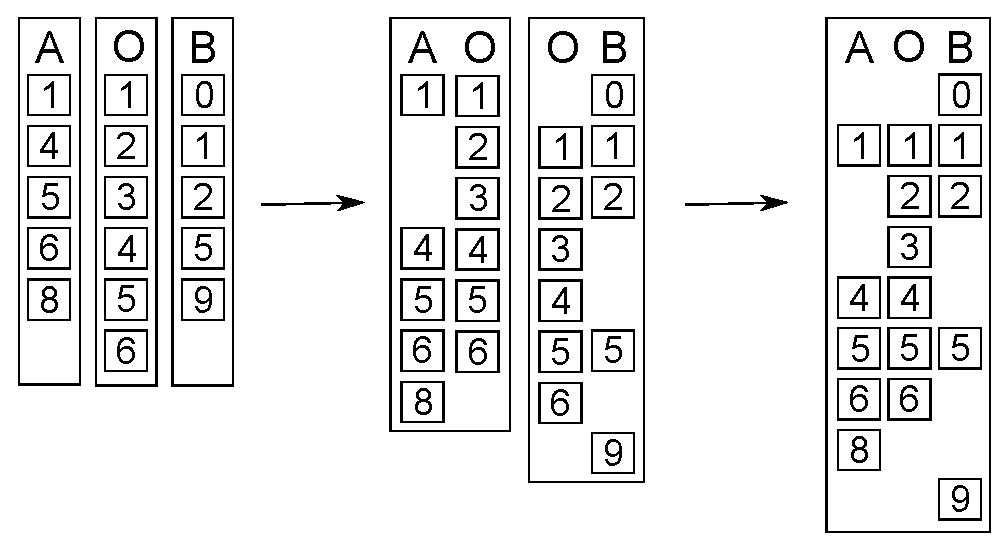
\includegraphics[scale=0.4]{drawings/eps/threewaymatching.eps}}
   \caption{A run of the Three-way matching-algorithm}
   \label{ThreewayMatching}
\end{wrapfigure}

Given three input sequences A, O and B it will often be necessary to match these structure, and output a single sequence of matchings between the three sequences. A match is a data-structure, that contains three elements A, O and B, illustrated as a row in the result of Figure \ref{ThreewayMatching}. An empty result in any of the three columns on each row means that there is no matching from this specific input sequence.

We will run two-sequence way matching two times on the sequence-pairs (A, O) and (O, B). Afterwards we will run a two way-matching on these two results, where equality between two two-way matches is defined as them not having an empty O-item, and having equal O-items. This will in the end giving us a list of matchings. The psudocode can be seen in Algorithm \ref{ThreeWayMatchingAlgorithm}.


\todo{Running time?}
\todo{Describe and illustrate problems with ambigious results}

\begin{algorithm}
\begin{algorithmic}
\Function{ThreeWayMatching}{$A$, $O$, $B$, $equality$}
	\State $AMatching\gets TwoWayAllign(A, O, equality)$
	\State $BMatching\gets TwoWayAllign(B, O, equality)$
	\State \Return $TwoWayAllign$($AMatching$, $BMatching$, $(x, y)$ $\Rightarrow$
        \State ~~~~ $x.O$ is not empty \and
        \State ~~~~ $y.O$ is not empty \and
        \State ~~~~ $x.O$ is equal to $y.O$
\EndFunction
\end{algorithmic}
\caption{The function for three-way sequence matching}
  \label{ThreeWayMatchingAlgorithm}
\end{algorithm}

\subsubsection{Chunking}
Given a three-way sequence matching, a single match can be defined as stable or unstable depending on whether or not all items $A$, $O$ and $B$ are present. This notion is quite useful for doing an actual merge. It is reasonable the assume that any stable match, does not not need to be merged.

\begin{wrapfigure}{r}{0.5\textwidth}
   \centerline{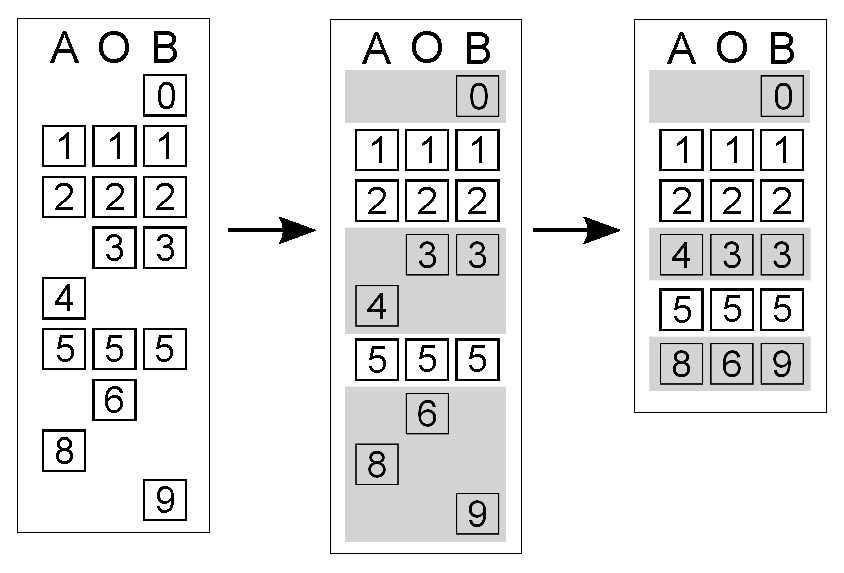
\includegraphics[scale=0.4]{drawings/eps/threewaymatching-chunking.eps}}
   \caption{Chunking a matching. Grey areas are unstable chunks and white areas are stable.}
   \label{Chunking}
\end{wrapfigure}

Another assumption one could make is that an unstable match can be viewed as either a deletion or an insertion. This however leaves us in a situation where all matchings can easily be resolved into a merge. This tells us something is inherently wrong with the approach. The problem lies in the fact that the matching sequence cannot represent the actual sentiment of the changes it is seeing: A deletion followed by an insertion might very well be an update of a single line. If both branches have done an update of the same line, then a conflict should be produced. Because of this we need to introduce chunking.

A chunk is three lists, one for A, one for O and one for B. A chunk can be stable or unstable. Given a sequence matching, we will generate chunks by iterating over every single match. If the first element is stable, then we generate a stable chunk, and add it's three items to the appropriate list. We continue adding all elements until we hit an unstable match. When we hit an unstable match we generate an unstable chunk, and add all non-empty elements from the match to the appropriate list.

The pseudocode for this algorithm is in Algorithm \ref{CunkingAlgorithm}. \footnote{The ChunkBy method used in the algorithm can be found at \url{http://msdn.microsoft.com/en-us/library/cc138361.aspx}}

\todo{Running time?}
\todo{Describe and illustrate problems with ambigious results}

\begin{algorithm}
\begin{algorithmic}
\Function{Chunking}{$matching$}
	\State $cs \gets matching.ChunkBy($no items in a matching are null$)$
	\State $chunks \gets []$
	\ForAll{$c$ in $cs$}
		\State $chunk \gets init new chunk$
		\ForAll{$m$ in $c.matches$}
			\If{$m.A \neq NULL$}
				\State $chunk.A.Add(m.A)$
			\EndIf
			\If{$m.O \neq NULL$}
				\State $chunk.O.Add(m.O)$
			\EndIf
			\If{$m.B \neq NULL$}
				\State $chunk.B.Add(m.B)$
			\EndIf
		\EndFor
	\EndFor
	\State \Return chunks
\EndFunction
\end{algorithmic}
\caption{Chunking algorithm}
  \label{CunkingAlgorithm}
\end{algorithm}


\subsubsection{Priority-chunking}
\label{PriorityDiff}
Our three-way matching function operates on equality. Yet in some cases we will actually want to use heuristics functions that define equality as a heuristic measure - as a similarity function - and pass this the the matching. This creates the problem that the heuristic equality function will not be able to distinguish between equality and similarity. Yet we want to make sure that completely equal inputs are matched before similarity is used - to get the most accurate results.

The solution to this problem will be priority-chunking as shown in Algorithm \ref{PriorityChunk}. It will start by doing a matching on the three input sequences using a strict equality function. It will then iterate through all chunks and for unstable chunks it will do another matching using the similarity-function. It will therefore generate three types of chunks:

\begin{itemize}
   \item Equality-stable items
   \item Similarity-stable items
   \item Unstable items
\end{itemize}

\begin{algorithm}
\begin{algorithmic}
\Function{PriorityChunk}{$A$, $O$, $B$, $equal$, $similar$}
	\State $matches \gets ThreeWayMatching(A, O, B, equal)$
	\State $chunks \gets Chunking(matches)$
	\State $outChunks \gets []$
	\ForAll{$chunk$ in $chunks$}
		\If{$chunk$ is stable}
			\State add $chunk$ to $outChunks$ as equality-stable
		\Else
			\State $innermatches \gets ThreeWayMatching $
			\State ~~~~~~~~~~~~~~~~~~~~~~~~~~~~ $ (chunk.A, chunk.O, chunk.B, similar)$
            \State $innerchunks \gets Chunking(innermatches);$
			\ForAll{$innerchunk$ in $innerchunks$}
				\If{$innerchunk$ is stable}
					\State add $innerchunk$ to $outChunks$ as similar-stable
				\Else
					\State add $innerchunk$ to $outChunks$ as unstable
				\EndIf
			\EndFor
		\EndIf
	\EndFor


	\State \Return outChunks
\EndFunction
\end{algorithmic}
	\caption{The algorithm for priority-chunking}
	\label{PriorityChunk}
\end{algorithm}


\subsubsection{Two-way set matching with costs}
Finding a minimum cost matching of the bipartite sets \texttt{x} and \texttt{y} can be solved in cubic time using a maximum flow algorithm as described by \citet{bipartitecost}. A prerequisite of this algorithm is however that the two sets are equal in size. Further, it assumes that the input can generate a perfect matching in the internal graph. We want to modify the bipartite graph algorithm such that it will be able to consume differently sized sets, and such it will generate the best minimum cost matching, even though it might not be a perfect matching.

The \citet{bipartitecost} algorithm starts by generating a weighted undirected graph, $G$. In this graph each item of the input sets is a node in the graph, and for each pair of nodes an edge is generated with the cost between them as the weight. The algorithm defines a set of prices $p$ for for each nodes. For $x$-nodes the initial prices are initially 0 and for $y$-nodes the initial prices is equal to the minimum weight of the incoming edges. It then creates an residual graph $G_M$ given a matching. The residual graph contains all the nodes of the original graph $G$, and further a source node $s$, and a sink node$t$. The source node has zero-cost edges to all $x$-nodes not in the matching and each $y$-node has a zero-cost edge towards the sink not in the matching. For each edge in the original graph, we will add an edge in the residual graph - if this specific edge exists in the matching we will add it as an edge from $y$ to $x$, otherwise from $x$ to $y$. The price weight of these edges will be the $price(xnode)+originalgraphweight-price(ynode)$. For each iteration of the algorithm it will update the prices such that the price in the next iteration is the current price and the cost to get from source to this node in the current residual graph.

The pseudocode for the algorithm can be found in Algorithm \ref{OriginalCostMatching}.


\begin{algorithm}
\begin{algorithmic}
\Function{OrgCostSetMatching}{$X$, $Y$}
	\State Generate $G$ from $X$ and $Y$ given a cost function
	\State Start with $M$ equal to the empty set
	\State Define $p(x)$ for $x \in X$, and  $p(y) = \underset{e \; into \; y}{\operatorname{min}} c_e$ for $y \in Y$
	\While{$M$ is not a perfect matching}
    	\State Find a minimum-cost $s-t$ path $P$ in $G_M$ with prices $p$
    	\State Augment along $P$ to produce a new matching $M'$
    	\State Find a set of compatible prices with respect to $M'$
    \EndWhile
	\State \Return $M$
\EndFunction
\end{algorithmic}
	\caption{The original cost-matching algorithm for sets.}
	\label{OriginalCostMatching}
\end{algorithm}

We want to modify this algorithm to have the following properties:

\begin{itemize}
\item It works for x and y sets of different size. 
\item It works even though a perfect matching cannot be found in the residual graph.
\item For any element not matched it should return a matching $(x, \epsilon)$ or $(\epsilon, y)$
\end{itemize}

If the sets are not equal in size, we will add nodes, auxiliary nodes, in the smallest of the two sets until the two sets are equal in size.\footnote{This concept is derived from a project I did in autumn 2012 with Torben Andersen} For each auxiliary node we will add an edge to each node in the opposing set with a cost larger than the largest cost between any other pair of nodes. In the final matching, the matchings that contain auxiliary nodes should be considered as not matched; since they have been matched with the highest possible weight for their edges - the rest of the matchings are definitely the minimum cost matching.
\todo{Forklar det her bedre}

The second challenge is due to the fact that the end-condition in the loop requires a perfect matching. However if any node in any of the two sets does not have a cost defined for a single node in the opposite set, then a perfect matching is not possible. An example of such a situation could be $X={1, 2}$ and $Y={1, 3}$ with a cost function only defined for elements that are numerically equal. This is demonstrated below. \\

\begingroup
    \fontsize{7pt}{10pt}\selectfont
\begin{tabular}{ p{5.5cm} | p{5.5cm} }
   \centerline{\includegraphics[scale=0.3]{drawings/eps/TwoWayCostMatchingNotPerfect/1it0.eps}} &
    \centerline{\includegraphics[scale=0.3]{drawings/eps/TwoWayCostMatchingNotPerfect/1it1.eps}} \\
   Initial graph for the sets and cost function. &
    The first residual graph. \\ \\ \hline \\

    \centerline{\includegraphics[scale=0.3]{drawings/eps/TwoWayCostMatchingNotPerfect/1it2.eps}} &
    \centerline{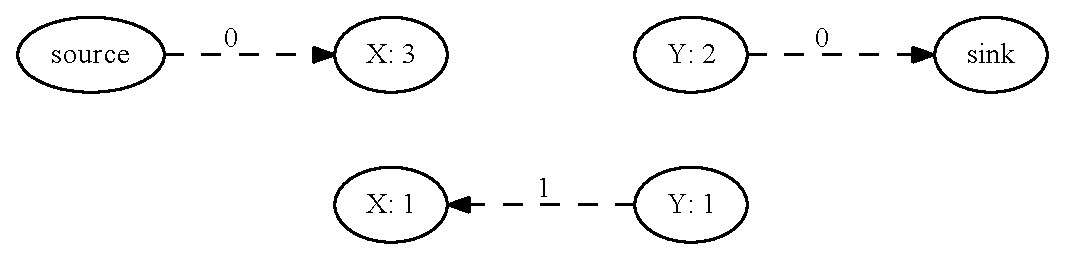
\includegraphics[scale=0.3]{drawings/eps/TwoWayCostMatchingNotPerfect/1it3.eps}} \\
   Running dijkstra finds a matching. &
   In the second residual graph, all possible matchings have been found, but the matching is still not a perfect matching. \\ 
\end{tabular}

\endgroup

When our algorithm reaches the second iteration, the matching is still not perfect for the entire graph. The problem is that one or more edges have no edges in the initial graph. The solution seems to be to not generate node with no costs generated for them, and return them as matchings with an empty opposite. This would obviously be a correct assumption; since they have no costs associated to the other set, they are of course impossible to match.

Looking at the same example, now that the node $(X: 1)$ actually has a cost to the node $(Y: 2)$. For this graph a perfect matching is not possible either. This situation is overcome by the generation auxiliary nodes after nodes with no cost have been deleted. As seen in the right figure below. \\

\begingroup
    \fontsize{7pt}{10pt}\selectfont
\begin{tabular}{ p{5.5cm} | p{5.5cm} }
   \centerline{\includegraphics[scale=0.3]{drawings/eps/TwoWayCostMatchingNotPerfect/NoFakeNode.eps}} &
    \centerline{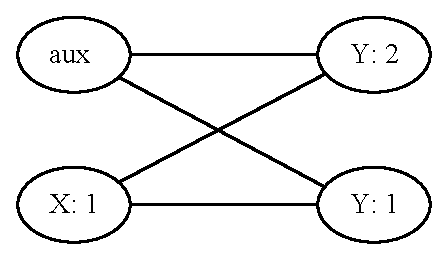
\includegraphics[scale=0.3]{drawings/eps/TwoWayCostMatchingNotPerfect/FakeNode.eps}} \\
   A graph where all nodes have a cost, but where no perfect match is possible. &
    The same graph, with auxiliary nodes added to make a perfect match possible. \\ 
\end{tabular}

\endgroup

We now have three sets, that together will be give the final matching:
\begin{itemize}
   \item The matchings that have an original input item in both ends.
   \item The matchings that have an auxiliary node in either end.
   \item The set of $X$- and $Y$-nodes that were never added to the graph.
\end{itemize}

We will simply union these sets and create matchings with an empty end apprioriately for the last two items in the list. The algorithm can be seen in Figure \ref{TwoWayCostMatching}.



\begin{algorithm}
\begin{algorithmic}
\Function{CostSetMatching}{$X$, $Y$}
	\State Generate $G$ from $X$ and $Y$ given a cost function.
	\State ~~~~ Store items of $X$ and $Y$ that has no cost.
	\State ~~~~~~ Do not add them to $G$.
	\State ~~~~ Inserting auxiliary nodes if the $|X| \neq |Y|$


	\State Start with $M$ equal to the empty set
	\State Define $p(x)$ for $x \in X$, and  $p(y) = \underset{e \; into \; y}{\operatorname{min}} c_e$ for $y \in Y$
	\While{$M$ is not a perfect matching}
    	\State Find a minimum-cost $s-t$ path $P$ in $G_M$ with prices $p$
    	\State Augment along $P$ to produce a new matching $M'$
    	\State Find a set of compatible prices with respect to $M'$
    \EndWhile
    

	\Return the union of three sets:
    \State ~~~~ For matchings with an auxiliary node, select $(x, \epsilon)$ or $(\epsilon, y)$
    \State ~~~~ For other matchings select the matching.
    \State ~~~~ For each item not added to $G$, select $(x, \epsilon)$ or $(\epsilon, y)$    
\EndFunction
\end{algorithmic}
\caption{The modified set matching function.}
\label{TwoWayCostMatching}
\end{algorithm}

\todo{Running time?}

\subsubsection{Three-way set matching with costs}
When we are given an original set $O$ and two branched sets $A$ and $B$, three way cost-matching will allow us to decided what items of each set belong together if we define a decent cost-function. 

Algorithm \ref{ThreeWayCostMatchingAlgorithm} will do two two-way matchings between $A$ and $O$ and between $O$ and $B$, and afterwards do a cost-matchings on these two matchings, where a cost is defined between the matchings if the $O$-item of each matching is not, and if they are equal.

\todo[inline]{We could probably just sort them after $O$-items, and then do a zipping on most of the lists.}

\begin{algorithm}
\begin{algorithmic}
\Function{ThreeWayCostMatching}{$A$, $O$, $B$, $cost$}
	\State $AMatching\gets TwoWayCostMatch(A, O, cost)$
	\State $BMatching\gets TwoWayCostMatch(B, O, cost)$
	\State \Return $TwoWayCostMatch$($AMatching$, $BMatching$, $(x, y)$ $\Rightarrow$
        \State ~~~~~~~~~~~~~~~~ $x.O$ is not empty \and
        \State ~~~~~~~~~~~~~~~~ $y.O$ is not empty \and
        \State ~~~~~~~~~~~~~~~~ $x.O$ is equal to $y.O$
\EndFunction
\end{algorithmic}
\caption{Three-way cost-matching algorithm}
  \label{ThreeWayCostMatchingAlgorithm}
\end{algorithm}

An over approximation of the running time here will be  $3*max(x, y, z)^3$.


\subsubsection{Reordering}
\label{ThreeWayReorderingAlgorithmSec}
Several times in this thesis, we will have matched sets together like they have no order, and will afterwards want to produce a sequence for our output. Here we will provide a function to resolve the problem where reordering of items in a sequence have happened in different branches. We will define a general three-way sequence-reordering-function, that can be given an original sequence and two reordered sequences, the result will be a single sequence where all elements are outputted in a way that can reasonably be described as a merge of the orders in the three input sequences.

Reorderings can conflict. One example could be that the sequence \texttt{(a, b, x, c, d)} has turned into \texttt{(x, a, b, c, d)} in one branch and \texttt{(a, b, c, d, x)}. These three sequences can easily be intepreted as \texttt{x} being been moved different places in the two branches, and a conflict should be produced.

If one branch moves an item and the other branch deletes it, we will intepret this as a deletion. The intuition behind this, is that generally unordered sequences in programming languages will be semantically meaningless. Therefore if one user deleted it while another user moved it, chances are that the item is not needed anymore, and can be deleted.

To do a three-way reordering, the obvious entry point is to identify which items have been moved, and then apply all these moves to the output sequence. This however leads to quite a few non-trivial definitions. What is a move? It might very well be an item of the sequences, but how do we define the place that it should be moved to? Several options are available: Insert after or before a specific item, insert between items or insert at index, and many more. Each of these items, however will also present further complications. If we choose to insert something after an item, in the output sequence, then do we do that before or after we move that item?

Further, such a move operation is not our input, and it is not clear how to calculate one from our input. Our input is three sequences with a specific order, and given those, many different move operations could be generated. The two sequences \texttt{a, b, c, d} and \texttt{a, b, d, c} can be interpreted as \texttt{c} being moved to after \texttt{d}, as \texttt{d} being placed before \texttt{c}, as \texttt{c} and \texttt{d} swapping places, and many other options. Also, figuring out the correct representation of a move in an algorithmic way can only be an uninformed guess - the users reasoning for doing a reordering might very well be grounded in context that the algorithm is unaware of.

We will look differently at reorderings. Given the input sequences we will do a matching. Such a matching will produce the actual ordering. We have earlier described small weaknesses in this approach, due to sequence alignment having more than one result, but will abstract away from that problem in this section.

A matching will contain some stable elements, and some unstable elements. The stable elements are elements where a match exists in both A, O and B. These elements, we will assume to be items that have not moved in the sequence. If something is not stable, it is either a move, an insertion or a deletion as seen in Table \ref{ReorderingTable}.

\begin{figure}
\centering
\begin{tabular}{ | l | l | l || r |}
  \hline                        
   \textbf{A} & \textbf{O} & \textbf{B} & \textbf{Action by user} \\
  \hline                        
  Empty & Value & Value & "Moved from" or deleted in A \\
  Value & Value & Empty & "Moved from" or deleted in B \\
  Value & Empty & Empty & Inserted or "moved to" in A \\
  Empty & Empty & Value & Inserted or "moved to" in B \\
  Value & Value & Value & Unchanged \\
  \hline  
\end{tabular}
  \caption{How to interpret matchings in the reordering algorithm}
\label{ReorderingTable}
\end{figure}

We will iterate through each matching, and treat them as such. Distinguishing between a deletion or a "move from" is not important - we will always treat them the same: Not adding them to the output. Distinguishing between insertion and moving is quite important however. Insertions should always be inserted in the output, however moves should only be inserted to the output if they have not been deleted in the opposite branch. 

A conflicting move is a move where two "Moved to" operations exists on each list. Detecting these is a matter of looking into duplicate records in the result list. These will also be returned along with the result, and the callers of the reordering methods have the responsibility of presenting these to the user.
\todo[inline]{Running time?}

\begin{algorithm}
\begin{algorithmic}
\Function{Reordering}{$A$, $O$, $B$}
   \State $matches \gets ThreeWayMatcing(A, O, B, items equal)$
   \State $resultList \gets []$
   
   \ForAll{$match$ in $matches$}
      \If{$match$ is insertion}
         \State add relevant item (A or B) to $resultList$.
      \EndIf
      \If{$match$ is move and exists in opposite branch}
         \State add relevant item (A or B) to $resultList$.
      \EndIf
      \If{$match$ is unchanged}
         \State add item O to $resultList$
      \EndIf
	\EndFor
	\State $conflicts \gets$ find indexes of duplicate items in $resultList$
	\State \Return $(resultList, conflicts)$
\EndFunction
\end{algorithmic}
\caption{Three-way reordering-algorithm}
  \label{ThreeWayReorderingAlgorithm}
\end{algorithm}

\subsection{Merging files}
Merging files will initially be done using a normal line-based approach, and when a conflict is detected, we will start breaking down the syntax tree and use this instead. In this section I will briefly describe our algorithms for the line based approach and for conflict detection and resolving.

\subsubsection{Sequence based merging}
The sequence based merging algorithm in figure \ref{Genericmergingalgorithm} is based on the description found of the original diff3 algorithm in \citet{Khanna}. Conflict Handling is delegated to an input function, to allow different handling in different situations. We pass the list of current merged text, and the currently unmerged chunk. The Merged list can be arbitrarily modified inside the conflict handler. Also, We allow the conflicthandler to break out of the entire loop. This gives allows for two essential use-cases:

\begin{itemize}
   \item Output the three items of the chunk, indicating that these are conflicting.
   \item Clear the merged list inside the conflicthandler, and start over with a different merging algorithm.
\end{itemize}


\begin{algorithm}
\begin{algorithmic}
\Function{Merge}{$A$, $O$, $B$, $equality$, $comparer$}
   \State $match  <- ThreeWayMatch(A, O, B, equality)$
   \State $chunks <- getChunks(match, comparer)$
   \State $merged <- []$
   \ForAll{$chunk$ in $chunks$}
        \If {$chunk$ is stable}
            \State add line of chunk.O to merged
            \State continue to next iteration
        \EndIf
        \If {$chunk$ is added in $A$ or $B$}
            \State add lines of $chunk$ to $merged$
        \ElsIf
            \If{$O$ is equal with one branch, but not the other}
               \State add lines of changed branch to $merged$
            \ElsIf
                \If{the two branches are equal}
                   \State add either of them to merged
                \ElsIf
                   \State $conflicthandler(merged, chunk)$
                   \If{$conflicthandler$ indicates termination}
                      \State break
                   \EndIf
                \EndIf
			\EndIf
   		\EndIf
    \EndFor
	\State \Return $merged$
\EndFunction


\end{algorithmic}
\caption{Generic merging algorithm}
  \label{Genericmergingalgorithm}
\end{algorithm}

\subsubsection{Mergefile function}
This $MergeFile$-function in Algorithm \ref{Mainmerge} will to do a line-based merge. It will do a syntactic merge if a conflict is detected in the file.

The main merging function of this thesis consists of a conflict-handler function and a general merge function. The merge function is passed in three lists of strings. Each item in this list represents a line in the code-files we want to merge. It will pass these lists to the to the sequence merging algorithm, and if this algorithm encounters a conflict, the conflicthandler will be called. The conflict-handler will empty the output, and launch the Syntax-aware merging, and add this as output instead. Then it will indicate to merging algorithm that this should return immediately.

\begin{algorithm}
\begin{algorithmic}
\Function{MergeFile}{$A$, $O$, $B$}
   \State $Conflicthandler \gets (output, chunk) \Rightarrow$
      \State ~~~~~~~~~~~~~~~~~~~~ clear $output$
      \State ~~~~~~~~~~~~~~~~~~~~ let $output$ be the result of $MergeSyntax(A, O, B)$
      \State ~~~~~~~~~~~~~~~~~~~~ terminate outer merge function
	\State $equality \gets (x, y) \Rightarrow x = y$
	\State \Return $Merge(A, O, B, equality, conflicthandler)$
\EndFunction
\end{algorithmic}
\caption{The main entry point for merging files}
  \label{Mainmerge}
\end{algorithm}

\subsection{Syntactic breakdown}
At some point we will have to break down the files from text to syntax trees. To do this we'll use Microsofts Roslyn Compiler. It has implemented a C\# syntax tree as a .NET class hierarchy, and with a single function call it is possible to get a syntax tree produced from a code file. This syntax tree seems to be very close corresponding to the actual grammatical rules set up by it's languages.


\todo{Write more about this}
\todo{Why C\#?}

\subsection{Merging classes}
\label{mergingclasses}
The top level of a C\# file contains an optional sequence of using-statements followed by a sequence of namespaces or type-declaration. A type-declaration is a struct, a class, an enum, a delegate or an interface. Classes, structs and namespaces can be nested in each other.

This structure in itself can lead to many potential merge scenarios; members of types can be moved and types can be nested in different way. We will look aside most of these issues and focus on merging purely inside classes. This means that a move of a class member will look like a deletion at one place, and an insertion at another place. As a consequence, a change in a function that is also moved moved between structures will therefore produce a conflict.

We do an unordered match between the the base file, and the two input brances using heuristics to determine the match. Nodes that are matched in the syntax trees are merged together. The overall process will be:

\begin{itemize}
   \item Match similar namespaces together and merge these.
   \item During a merge of namespaces, match similar classes together and merge these.
   \item During the merge of classes, match similar class-members merge these.
\end{itemize}

The input for the Algorithm \ref{TreeMergeAlgorithm} is three syntax tree generated from the input files. The output is a text string with the concrete syntax of the merge. Whenever the function encounters a namespace or a class, we will do an unordered matching on these, and recursively call itself for each match. Whenever a class-member is hit in the recursive call, we will try a line-based merge. If a conflict happens during this merge, we will launch a syntax based merge of the specific class-member. The effect of this is, that class-members will be only be doing expensive syntax merge as a last resort.

After creating the merge of all children for a class or a namespace, we need to create the ordered sequence of the merged items, that can be used to generate the entire merged node. We store all matches in a list, along with their merge-result. From this list we will generate three new sequences for each input sequence. These lists will be feeded into the reordering function seen in section \ref{ThreeWayReorderingAlgorithmSec}.

One extra detail is needed however. Items that are deleted in one branch, and modified in another branch, should generate a conflict. The reordering function assumes equality between the items in the sequences, and therefore cannot consider a deletion to be a possible conflict. Therefore we will have to detect conflicts during merging and pass a set of these to a modified Reordering function, that will only delete items, if they are not a part of this set.

\begin{algorithm}
\begin{algorithmic}
\Function{MergeSyntax}{$A$, $O$, $B$}
    \If{nodes are roots, namespaces or classes}
        \State $zip  \gets ThreeWayCostMatching(A, O, B, $ relevant cost function $)$
        \State $members \gets [];$
        \State $deletionconflicts \gets []$
        \ForAll{$match$ in $zip$}
           \If{$match$ exists in all}
               \State $member.add(match, MergeSyntax(A, O, B)) $
           \ElsIf{match was inserted in A or B}
              \State $member.add(match, (A or B item))$
           \ElsIf{match was deleted and changed in opposite branch}
               \State $member.add(match, (A or B item))$
               \State $deletionconflicts.add(A or B item)$
           \EndIf
           \State $reorderLists \gets $ map each item in each list (A, O, B)
           \State ~~~~~~~~~~~~~~~~~~~~~~~~~~~~~~~~~~~~~~~~~~~~ to their merged result.
           \State $members = Reorder(A, O, B, conflicts)$
       \EndFor
       \State \Return $recreate(b, l, r, members)$
    \ElsIf{nodes are classmembers}
       \State Run $MergeFile$ on the source text of A, O, B
       \State If a conflict happens run $MergeNode$ on the nodes.
    \EndIf
\EndFunction
\end{algorithmic}
\caption{The entry point for syntactic merge}
\label{TreeMergeAlgorithm}
\end{algorithm}

\subsubsection{Cost-functions}
We will have to define the cost-functions for namespaces, classes and class-members. For each level, these functions will be called for each pair of items possible in $(A, O)$ and $(O, B)$. As a consequence, it we will have to keep the runtime cost of calculating a cost of two items relatively low.

For classes and namespaces we will define functions that assign low cost to nodes with similar identifiers, and a higher cost to all other nodes of the same type on the same structural level. This approach has the benefit of being quite fast. Further, renaming a class on the same structural level, will have no consequence, since it will be just be matched to another node of the same type. A drawback, however, is that given this heuristic, we have no way to know what to do if a node has been renamed and another node inserted at the same time: All possible matchings in such case are valid and has the same cost. A better heuristic for namespaces and classes, would probably be to also include the different members of namespaces and classes as a part of the cost-function, however we decided not pursue this approach further.

One obvious function to use to assign the cost between two functions, would be the similarity function defined in section \ref{FunctionSimilarity}. However this function is quite intensive computation-wise, since it walks through the entire subtree. This would lead to an explosion in computation time for the overall matching algorithm\todo{Running time}, since it is done for every possible pair. Instead we will limit our matching to the signature of a method:

\begin{itemize}
    \item The return type.
    \item The identifier.
    \item The type and identifier for each parameter.
\end{itemize}

The more of these factors that are similar, the lower a cost two functions should have. Matching functions that are very dissimilar in their method body might produce unproductively amounts of conflicts, and because of this it's a goal of this heuristic to not match things together too greedily.

Equal identifiers is a clear sign of similarity, and one that should weight heigh for this scale. Parameters are also important; we need to match different overloads of a function to the same overload in another branch. Given these two criterias we will match any unchanged function completely.

If we are looking at two functions with dissimilar names, equal return types and no parameterlist, it is not quite obvious how to define if they are similar or not. For this reason we will define it as not similar. However with several parameters similar, the likelihood of the functions actually being the same increases.  The cost-function can be found in Algorithm \ref{MethodCostFunction}.
\begin{algorithm}
\caption{The Cost-function for methods}
\label{MethodCostFunction}
\begin{algorithmic}
\Function{FunctionCost}{x, y}
   \State $parametersimilarity \gets 0$
   \If{parameterlists of $x$ and $y$ are not empty}
      \State match parameters after having either identifier or type equal.
      \ForAll{$match$}
	      \State select 1 if both name and type are equal
    	  \State select 0.5 if either name or type are equal
	      \State select 0 if there is no matching item
      \EndFor
      \State $parametersimilarity \gets 4*the averager of above match value$
   \EndIf
   \State $cost \gets 9$
   \If{equal return type of $x$ and $y$}
      \State $cost \gets cost - 1$
   \EndIf
   \If{equal identifiers}
      \State $cost \gets cost - 4$
   \EndIf
   \State $cost \gets cost - parametersimilarity$
   \If{$cost \geq 4$}
         \State \Return No link
   \EndIf
   \State \Return $cost$
\EndFunction
\end{algorithmic}
\end{algorithm}

This function has some properties that are helpful, given the above considerations:

\begin{enumerate}
\item If the name of a function is equal, a possible match will be produced.
\item Higher similarity between parameters gives better costs.
\item Renamed functions can be matched if they match completely in the parameterslist, or if some of the parameterlist is similar and it has the same return type.
\end{enumerate}


\subsection{Merging functions}
\todo[inline]{Foreach function, write about:

- Intended input. \\
- Purpose of the function.\\
- Conflict behaviour\\
- Tricks that are not obvious.\\
- Intended output.\\}

\subsubsection{Merging nodes}
\texttt{MergeNode} handles merging of single nodes of equal type. It will take three input values; A, O and B, and return a syntactically valid string, which is the merge of those three input values. It handles the input as a matching and will conclude insertion or deletion if appropriate. Further it assumes that all input nodes are of the same type.

\begin{itemize}
   \item If O is null and either A or B is null it treats the input as an insertion, and returns the inserted value.
   \item If O is not null, and A or B is null it treats the input as a deletion. It will verify that no changes has happened in the other branch and return either a conflict, or empty.
\end{itemize}

Otherwise it will treat the input as a merge of the two branches A and B. From a concrete syntax perspective, we will have to look into two factors of the current node, to see what to return:

\begin{itemize}
   \item The concrete syntax that this node emits.
   \item The concrete syntax that each child of this node emits.
\end{itemize}

The responsibility of an invocation of MergeNode is to return the the exact syntax needed for these specific node. Any work of generating concrete syntax for children will be handled by a recursive call to MergeNode. For example a method invocation will simply generate the opening and closing parenthesis, while the argument list will simply be passed to another invocation, as well as the method-expression. This breakdown makes the merging of most nodes quite trivial.

Some nodes only consists of tokens: A function name, a string literal, an integer, a keyword and so forth. For these kind of nodes, we will simply check if only one of the branch nodes differs, and if this is the case, return that, and otherwise return a conflict, as can be seen in Figure \ref{MergeToken}


\begin{algorithm}
\caption{A fixed structural node is nodes that has a fixed number of children, that are easily merged - like methods declerations, expressionsstatements, invocations, memberaccesses, single arguments. A content node is a node which is generated from a single token.}
\label{MergeNode}
\begin{algorithmic}
\Function{MergeNode}{$A$, $O$, $B$}
    \If{$A$ or $B$ has been deleted}
        \If{others havent changed}
            \State \Return nothing;
        \Else
            \State \Return conflict;
        \EndIf
    \EndIf
    \If{$A$ or $B$ has been inserted}
        \State \Return $A$ or $B$
    \EndIf
    \If{nodes are fixed structural nodes}
        \State \Return merge of each child and own structure
    \EndIf
    \If{node is a content-node}
        \State \Return $TokenMerge(A, O, B)$
    \EndIf
    \If{nodes is a list}
        \State \Return $Listmerger(A, O, B, $ appropriate cost function $)$
    \EndIf
    \If{node is a block}
        \State \Return $MergeStatementList(A.children, O.children, B.children)$
    \EndIf
\EndFunction
\end{algorithmic}
\end{algorithm}


\begin{algorithm}
\begin{algorithmic}
\Function{MergeToken}{$A$, $O$, $B$}
    \If{all equal}
        \State \Return value
    \EndIf
    \If{one has changed}
        \State \Return changed value
    \EndIf
    \If{both has changed}
        \If{$A \neq B$}
            \State \Return conflict
	    \EndIf
        \State \Return A
    \EndIf
\EndFunction
\end{algorithmic}
  \caption{Merging tokens}
  \label{MergeToken}
\end{algorithm}

\subsubsection{Equality}
The equality function will define whether or not two nodes taken from syntax-trees in different branches are equal to each other.

If we view syntax trees as simple n-ary trees with no semantic meeting, this becomes easy. Every node has a label and $n$ children. Given two nodes $x$ and $y$ we need to check if the label is equal, and we need to iterate through each pair of children on the same index. Whenever we encounter something not equal, return false. Otherwise return true.

\subsubsection{Similarity}
\label{FunctionSimilarity}
Similarity should return whether two nodes are similar or not. We will divide it into two functions:  One that decides a similarity percentage between two nodes. Around this function we will define a function that thresholds this percentage.

\paragraph{Initial assumptions} Is the expression $x=1+2+3$ similar to $f(1+2+3)$? They have atleast 5 nodes in common; three integers and two add operators - this, out of 7 nodes in total. From that perspective they seem quite similar. However, for several reasons, we will decide that only syntax-nodes of equal type should be considered similar:

\begin{enumerate}
\item As noted by \citet{Hashimoto}, showing a fine grained difference, might actually be more confusing than showing the two statements as an insertion and deletion.
\item The running time of creating the matchings, will become considerably larger if every single sub-tree will have to be compared to each other sub-tree for similarity.
\item The complexity of the merge algorithm will be considerable less, if we can assume that children of any of the input nodes are always the same. This would also be the case for the similarity function itself.
\item If we want to allow for merging of the above cases, this can still be done, in the same way that we allow of uneven tree merging when no other ways of resolving an update is possible: It will generate an unstable chunk. Given this chunk we can match the sub-trees much quicker because we have a much more narrow field for the matching.
\end{enumerate}

Given that two nodes are only equal if they are of the same node-type, most of the similarity will be quite straightforward: Run similarity on all children, and do an average of these. This is however not possible for nodes that contains lists of sub-nodes - blocks, parameter-lists and argument-lists.

\paragraph{Lists} There will exist lists of parameters and arguments throughout the syntax tree. Finding similarity between these lists, will be a question of matching the arguments or the parameters inside the lists. This matching we will do without order: If the order of parameters or arguments have changed across branches, it is probably more due to reorderings or change in overloads, than it has anything to do with change in actual behaviour.

\paragraph{Blocks} Similarity for blocks will be determined by doing a priority-chunk-matching, and for each chunk, count up by adding up the similarity and the count of statements:

\begin{itemize}
	\item For equality-stable chunks we will add 1 to the similarity and 1 to the statement-count foreach statement
	\item For similarity-stable chunks we will the similarity between the two statement, and 1 to the statement-count foreach matching
	\item For unstable chunks we will add nothing to the similarity and the maximum amount of statement in both of the sides for the unstable chunk.
\end{itemize}

The first two are obvious: Together they will be used to calculate the average similarity across statements. The 

\paragraph{Token similarity} Tokens-similarity, in this case integers and strings, can be defined in a few ways. 

\paragraph{Threshold}

\subsubsection{Merging lists}
There are primarily two types of list that we want to merge: ParameterLists and ArgumentLists. Parameterlists are the pair of types and identifiers found in method declarations, where argument-lists are expressions found in invocations of methods. Modification of these two properties 

\begin{itemize}
   \item Modifications of parameter-lists can be reorderings with no semantic meaning. Further it can be additions or removals of a parameter. These will often also be accompanied by some change in the behaviour of a method.
   \item Modifications of argument-lists can be done as a consequence of change in a parameter list other places in the syntax-tree. They can also be done simply because another expression or value needs to be passed into a function, or because the user intends to call another overload of the method.
\end{itemize}

The first part is solved the same way that we reorderings were solved in section \todo{page number}. We will do an unordered matching of them, and then do a reordering, and filtering of the output. The returned list is a list that tries to preserve any reordering, and that has filtered items in the sequence that did not exist in either of the two branches. This will hopefully ensure that:

\begin{itemize}
   \item Since the reordering uses the exact same algorithm a merge of parameter- and argument-lists will produce compatible output, given that the cost function matches in the same way on both branches.
   \item All items that existed in the branches will exist in the output of this function. 
\end{itemize}
The cost between a pair of parameters can be boiled down the question of how similar the type of the parameter is, and how similar the name is. Similarity of type can be measured as closeness in the class hierarchy. String similarity can be measured in quite a few ways. In our case we will want to keep the runtime low and as such we will keep to a simple and exact scheme of similarity of both.

The cost of the argument-lists is much harder to define. An argument is an expression, so the obvious thought would be to look into what type that expression will have. This information, however, is not available to us. Instead we will simply look into the string value of the nodes and compare these for equality or not. Lower equality means lower cost. This cost-function makes will produce matching of items that have not been changed, but have been reordered, and items that have changed will not be matched, and therefore be treated as insertions, deletions or moves.

The first item in the above list, depends on the matchings in both parameterlists and argumentlists to match the same items. This is not generally true for for the two matching functions that we provide, but it will be true in cases where reordering have happened without changing the expressions of each parameter.

\begin{algorithm}
  \caption{Merging unordered lists}
  \label{Listmerger}
\begin{algorithmic}
\Function{Listmerger}{A, O, B, cost}
    \State $match \gets ThreeWayCostMatching(A, O, B, cost)$
    \State $(merge, conflicts) \gets FilterReorderMergeContent(a, o, b, match)$
    \ForAll{conflict}
        \State Add a warning to the merges.
    \EndFor
    \State \Return $merge$
\EndFunction
\end{algorithmic}
\end{algorithm}

\subsubsection{Merging blocks}
A block-node is hit by the MergeNode algorithm often. They are the body of methods, if-statements, while-loops, using-statements and more. We need to merge content inside in each branch and the base. We will first try to do a textual merge of the content of the block. If this fails, we will do a priority-differencing as described in section \ref{PriorityDiff}, with the equality and and similarity function defined in Algorithm \ref{FunctionSimilarity}.

Given these chunks we will handle them in three different ways: 

\begin{itemize}
	\item If a chunk is Equality-stable use the input from the base tree.
	\item If a chunk is Similarity-stable, merge each node using $MergeNode$
	\item If a chunk is unstable, check of either branch is equal with base, and use the other.
	\item Otherwise try to do an uneven merge as described later.
\end{itemize}

\begin{algorithm}
  \caption{Merging statement lists}
  \label{MergeStatementList}
\begin{algorithmic}
\Function{MergeStatementList}{A, O, B}
    \State try  a textual merge of the statements.
    \If{that does not work}
        \State $chunk \gets PriorityDiff(A, O, B, equality, similarity)$
        \ForAll{chunks}
            \If{chunk is primaryequal}
                \State \Return $chunk.O$
            \ElsIf{chunk is secondary equal}
                \State for each line \Return $MergeNode(A, O, B)$
            \ElsIf{either A and O or O and B are equal}
                \State add the opposite chunk.
            \Else
                \State attempt uneven merging
            \EndIf
        \EndFor
    \EndIf
\EndFunction
\end{algorithmic}
\end{algorithm}

\subsection{Merging uneven trees}
Generally our merge has been working with structural equality. This means that if one branch moved a chunk of code into a block, and the opposite branch changed something in the chunk of code, we have no way of handling this.

$MergeUneven$ is called in case of an unsolvable conflict in Algorithm \ref{MergeUneven}, and tries to handle the scenario of inserted sub-block in the code - for example wrapping a couple of lines of code in an if-statement. It takes an unstable chunk as input, that contains a sequence of nodes that cannot be matched. MergeUneven looks for nodes in the chunks that contains sub-blocks which might create a stable match. It works as can be seen in Figure \ref{UeventreeProcess}. Below is a description of each step.

\paragraph{Flattening} $MergeUneven$ will start by flatting the input lists, in the sense that for any node found in the input lists that contains a sub-statement or a block, we will bring these statements into the top level. During the flattening we will also remember the parent of each node, as can be seen in the left columns of the Flattened-item in the figure. Looking at the flattened list of child and parent elements,  it is obvious that chunks of continuous parent items in any of the three lists is a sub-block.

\paragraph{Matching} Afterwards we will run $PriorityChunking$ on the child elements of the flattened lists. If some statements have been moved to a subscope for these conflicts, this matching will match these statements with the ones in the other branches scope. As mentioned above, a continuous sequence of keys in the three branches means a sub-block. The same will be the case in this matching: For each branch, we will be able to track opening and closing sub-scopes by looking at the change between the last observed parent element, and at the current. This means we will be able to isolate chunks of matches that happen in specific scopes. After isolating these, we can merge the parents, and for each continuous sequence of parent items, we can output a block around them.

\begin{figure}
   \centerline{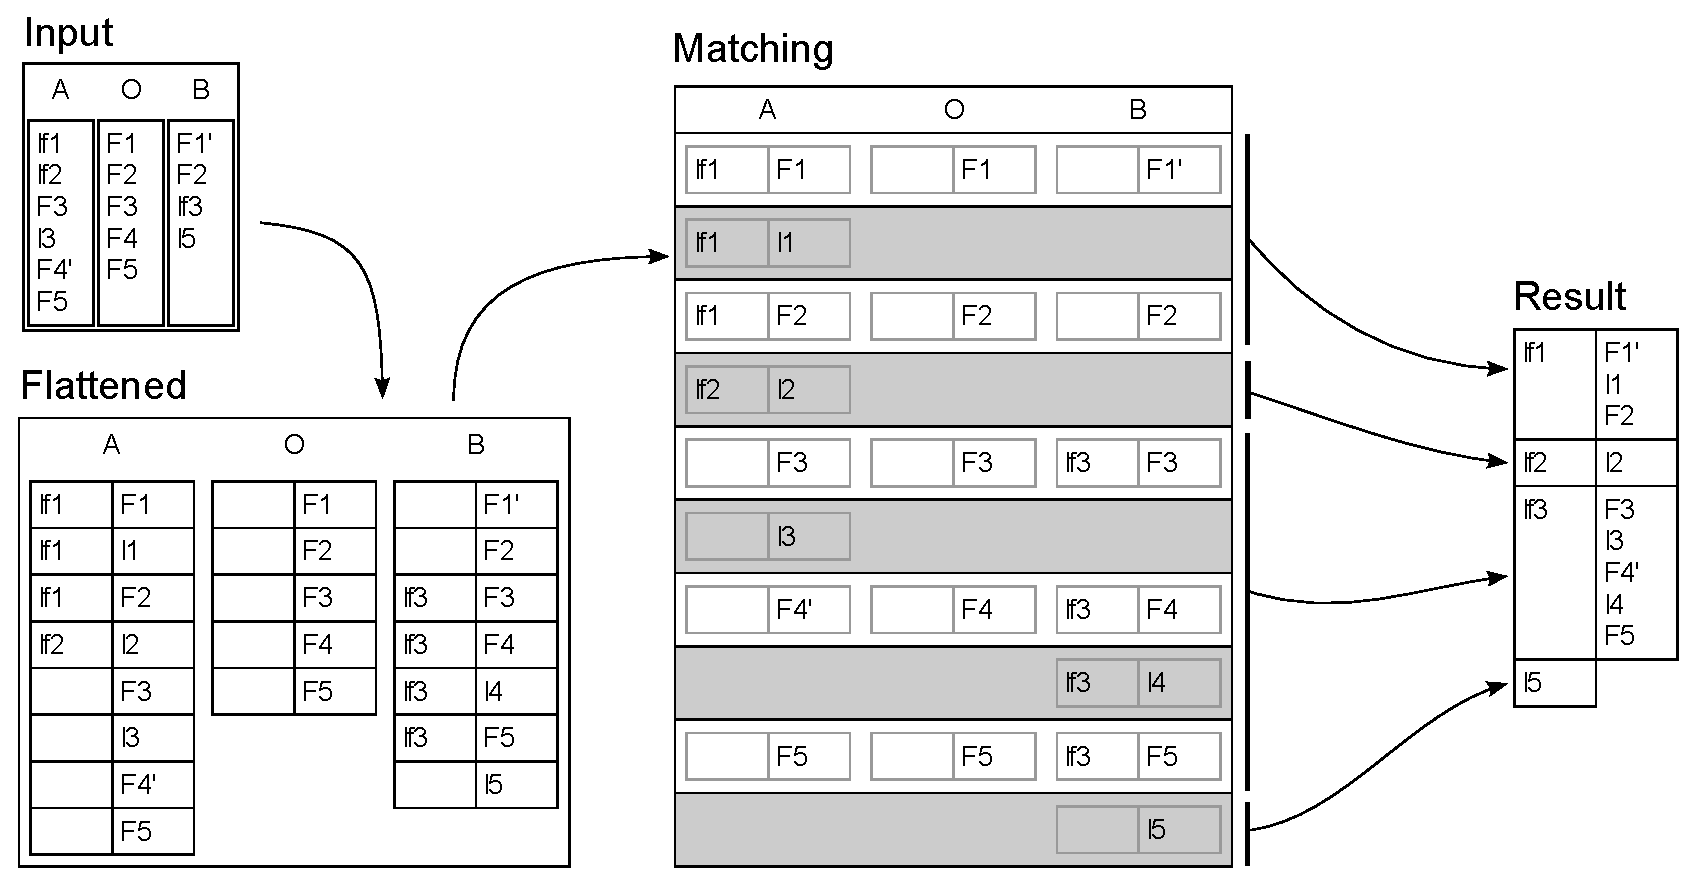
\includegraphics[scale=0.55]{drawings/html/EditedFlattenedMerge.eps}}
   \caption{Process of merging uneven trees.}
   \label{UeventreeProcess}
\end{figure}

\begin{algorithm}
\begin{algorithmic}
\Function{MergeUneven}{A, O, B}
    \State Flatten the three list. Any statement with a subblock, has the statements in this subblock added to it, keeping parent item mapping
    \State Prioritydiff the three flattened lists.

    \State Parentitems = [nil, nil, nil]
    \ForAll{$chunk$ in $chunks$}
        \If{$chunk$ is stable}
            \If{lastitem O is null and B and A is not}
                \State \Return conflict
			\EndIf
            \If{any parentitem has changed since last iteration}
                \If{last parent item as a block block}
                    \State print "\}"
                \EndIf
                \If{a current parent item exists}
                    \State print(merge(parentitems))
                    \If{currentparentitems merrits block}
                    	\State print "\{"
                    \EndIf
                \EndIf
			\EndIf
            \State print merge(child item)

        \ElsIf{$A$ or $B$ is insertion}
                \State add A or B, updating their corresponding parentitem,
                \State and adding starting and ending items, as above
        \EndIf
   \EndFor

\EndFunction
\end{algorithmic}
\caption{Merging uneven branches}
\label{MergeUneven}
\end{algorithm}


\clearpage
\section{Evaluation}

\clearpage
\section{Conclusion}

\clearpage

\bibliographystyle{plainnat}
\bibliography{libary}

\end{document}

